\documentclass[UTF8]{ctexart}
\usepackage{indentfirst}
\usepackage{graphics}

\title{人工智能 总结报告}
\author{佘天唯}
\setlength{\parindent}{2em}
\graphicspath{{./2014201972/figures/}}

\begin{document}
	\maketitle	
	
	\section{图像分类}
	\subsection{环境与框架(Week 1-2)}
	安装Linux系统
	
	安装Caffe:因为不使用GPU训练,没有安装CUDA等
	\subsection{学习CNN模型(Week 3)}
	局部感知,参数共享,多卷积核,池化操作
	\subsection{熟悉Caffe的使用(Week 4-5)}
	配置文件格式,网络Layer分类,训练实例模型(LeNet等),尝试Fine-tuning
	\subsection{搭建Residual Net模型(Week 6)}
		\subsubsection{网络结构}
		如He Kaiming残差网络论文中在Cifar10数据集上进行验证所构建的网络结构基本一致,如下图(其中$n=3$),得到20层ResNet网络
		\begin{figure}[htbp]
			\centering
			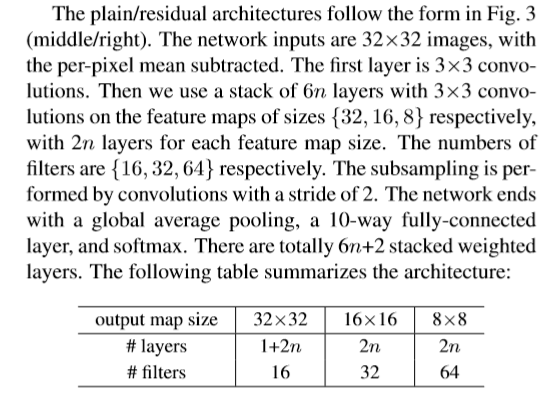
\includegraphics[scale=0.8]{1.png}
		\end{figure}
		
		\subsubsection{Shortcut Connections的实现}
		前一层的输出直接加到下一层,如图:
		\begin{figure}
			\centering
			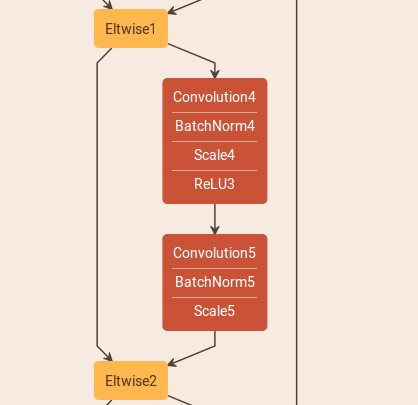
\includegraphics[scale=0.4]{2.png}
		\end{figure}
		
		\subsubsection{Dimension increase处的处理}
		Shortcut部分加一个卷积层,通过控制stride的大小实现,如图:
		\begin{figure}
			\centering
			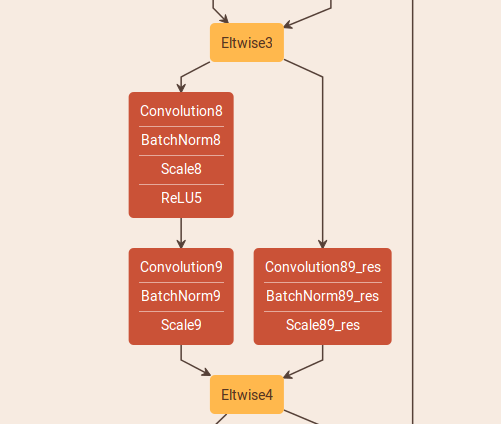
\includegraphics[scale=0.4]{3.png}
		\end{figure}
	\subsection{在Cifar10数据集上训练(Week 7)}
		网络配置文件:res20\_cifar10\_train\_test.prototxt
		
		训练参数配置文件:res20\_cifar10\_train\_test.prototxt
		
		训练效果:迭代至11100次左右准确率保持在75\%-80\%,如下图(没有GPU,在自己的电脑上跑,时间原因只迭代了11000次左右):
		\begin{figure}
			\centering
			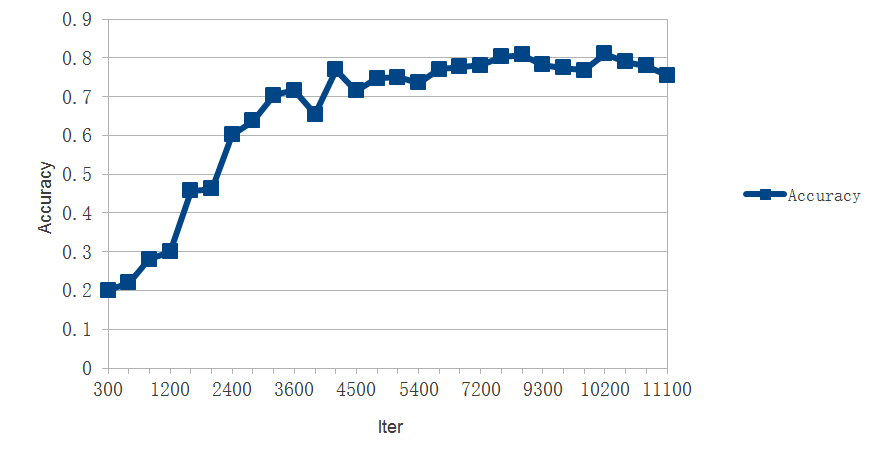
\includegraphics[scale=0.7]{4.png}
		\end{figure}
	
	\subsection{BOT数据集预处理(Week 8)}
		将接近5万张图片大体按$4:1$的比例分为训练集和测试集,生成记录所有图片路径及标签的txt文档
		
		用caffe自带工具将图片resize为$32*32$大小,并转化为lmdb格式,生成均值文件
	
	\subsection{在BOT数据集上训练(Week 9)}
	 	网络配置文件:res20\_BOT\_train\_test.prototxt(在之前Cifar10的ResNet基础上改掉输入data层即可)
	 	
	 	参数配置文件:res20\_BOT\_solver.prototxt(因收敛太慢,训练中途曾尝试更改learning rate policy,但效果不明显)
	 	
	 	训练结果:
	 	\begin{figure}
	 		\centering
	 		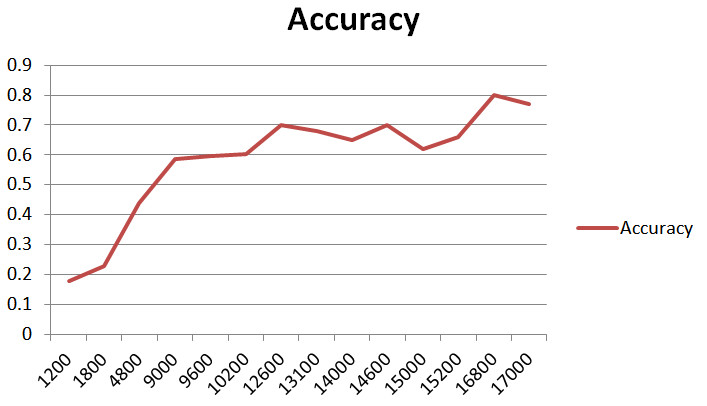
\includegraphics[scale=0.7]{5.png}	
	 	\end{figure}

	\section{文本分类}
	\subsection{文本分类入门(Week 1)}
	安装Tensorflow,跑了一个用CNN实现句子分类的代码,但没看懂...
	
	了解了文本分类的基本原理和步骤
	\subsection{文本数据集(Week 2)}
		\subsubsection{假论文}
		通过保存随机访问SCIgen并保存网页源码、用BeautifulSoup去除HTML标签的方式,爬取了1000篇假论文,存为txt格式
		
		代码:/code/crawl\_neg\_paper
		
		
		样例文本:/papers\_example/neg\_0.txt
		
		\subsubsection{真论文}
		将老师给的3800篇真论文用linux自带的pdftotxt命令/python的pdfminer包转化为txt格式
		
		样例文本:/papers\_example/pos\_0.txt
	
	\subsection{学习TensorFlow使用(Week 3)}
	实现了简单的CNN模型,在mnist数据集上训练,达到98\%正确率
	
	代码:mnist\_CNN.py
	\begin{figure}
		\centering
		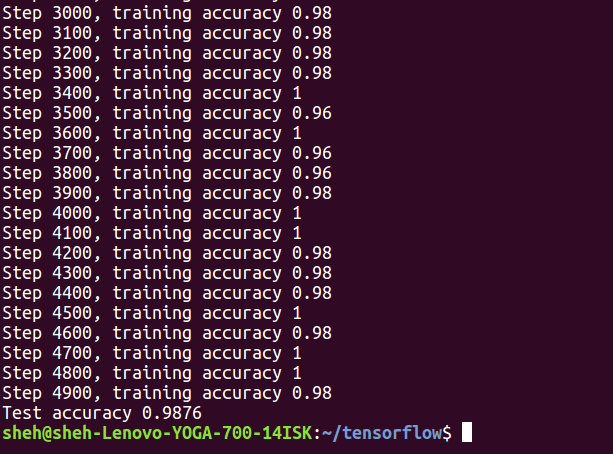
\includegraphics[scale=0.6]{6.png}	
	\end{figure}
	
	\subsection{文本预处理(Week 4)}
	去标点去数字,化小写,去停用词(从网上找的英文停用词表)
	
	代码:preprocess.py
	
	词频统计,得到每个文档出现次数最多的前300个词的出现次数作为输入特征
	
	代码:frequency.py
	
	样例文本:/papers\_example/neg\_1.txt; /papers\_example/pos\_1.txt	
	\subsection{SVM文本分类(Week 4)}
	使用libsvm工具,以前面生成的300维特征作为输入,用SVM模型训练预测,准确率达到99\%,如图:
	\begin{figure}
		\centering
		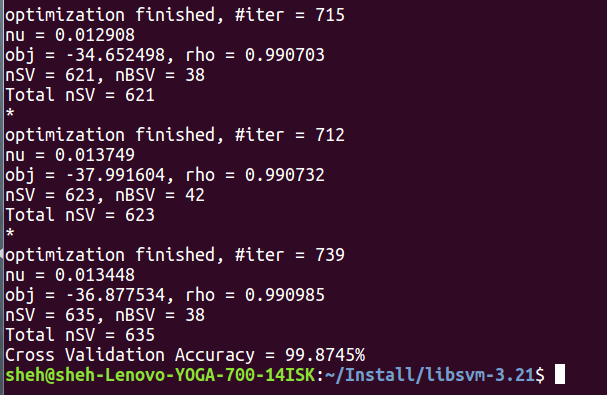
\includegraphics[scale=0.6]{7.png}	
	\end{figure}
	
	\subsection{使用TensorFlow搭建CNN文本分类模型(Week 5)}
	
	
\end{document}
